\documentclass[11pt, oneside]{article}   	% use "amsart" instead of "article" for AMSLaTeX format
\usepackage{geometry}                		% See geometry.pdf to learn the layout options. There are lots.
\usepackage[parfill]{parskip}    			% Activate to begin paragraphs with an empty line rather than an indent
\usepackage{graphicx}						% Use pdf, png, jpg, or eps§ with pdflatex; use eps in DVI mode
											% TeX will automatically convert eps --> pdf in pdflatex
\usepackage{amssymb}
\usepackage{hyperref} 						% for \hyperfootnote
\usepackage{pifont}							% for \ding
\usepackage{url}							% for "plainurl" support in \bibliographystyle 
\usepackage{comment}

% Make clickable footnote
\newcommand{\hyperfootnote}[1][]{\def\ArgI{{#1}}\hyperfootnoteRelay}
	% relay to new command to make extra optional command possible
\newcommand\hyperfootnoteRelay[2][]{\href{#1#2}{\ArgI}\footnote{\href{#1#2}{#2}}}
	% the first optional argument is now in \ArgI, the second is in #1
% Takes at most 3 parameters (see http://www.tex.ac.uk/FAQ-twooptarg.html for info on multiple optional parameters)
% If first parameter isn't given, it's value is '' (empty string in text before footnote reference)
% If second parameter isn't given, it's value is '' (string before visible URL, e.g. 'http://')
% Makes a clickable footnote (alternatively: \url{}) with optional reference in the text as well
% Use 1: \hyperfootnote{www.mywebsite.com}: creates a footnote consisting of a clickable URL
% Use 2: \hyperfootnote[My website]{www.mywebsite.com}: creates a clickable piece of text in the text ('My website') plus a footnote consisting of a clickable URL
% Note: requires the hyperref package.
% Note: use xspace package to add/absorb spaces when necessary (e.g. to avoid a space between the footnote number and a punctuation mark)
% Info on how to define a LaTeX command: https://www.sharelatex.com/learn/Commands

\geometry{letterpaper}                   	% ... or a4paper or a5paper or ... 
\usepackage{draftwatermark}
\SetWatermarkLightness{0.9}
\SetWatermarkText{DRAFT}					% you can use \today
\SetWatermarkScale{4}

\title{Age Protect}
\author{Paul Trevithick\footnote{The Mee Foundation}, Denise Tayloe\footnote{Privacy Vaults Online, Inc. dba PRIVO}, Alexander Yuhimenko\footnote{Swift Invention, Inc.}}
\date{May 29, 2023. Revised \today}							
\begin{document}
\maketitle
\begin{abstract}
	We present a new age verification approach with a unique combination of characteristics: (i) it is opt-in: a parent or guardian can choose to protect their minor children and adults can use it to prove they are of age (ii) the privacy and anonymity of all parties is respected (iii) it leaves the existing internet experience completely unchanged. Age Protect is a technical specifical that defines the interactions between three kinds of parties: online service providers, smartwallets, and AVSes. Service providers can implement it to offer age-restricted content and services consistent with prevailing laws and regulations. People can use it by installing a compatible on-device software smartwallet and having a relationship with an compatible Age Verification Service (AVS). Using this smartwallet a person can convey AVS-attested age-related information to service providers which can use it to authorize access to content and services they offer on their apps, websites, or other online services. 
\end{abstract}

\section{Introduction}

Society agrees to supervise the places children inhabit, protect them from environments they should not encounter, and regulate the products they use. Businesses are not permitted to sell tobacco, alcohol, pornography, handguns, certain kinds of fireworks, and other products and services to minors. None of this is true online. In the virtual world children are largely unprotected despite being exposed to wide range of potential harms. 

Many approaches have been proposed and tried without success. Existing laws have proven to be insufficient, and industry self-regulation has failed. There is a renewed global push to protect children's safety through stronger laws and regulations. Although some use other approaches\footnote{Such as requiring online services that are likely to be used by young people to default to the highest privacy setting possible for minors, as mandated by California's Age-Appropriate Design Code Act.} many mandate age verification.\cite{Griswold2023}\cite{Jackson2023} However, privacy advocates and others have shown that many of the mechanisms for verifying age online weaken anonymity and privacy.\cite{Roth2023} 

Age Protect is a new age verification solution with a unique combination of characteristics: (i) it is opt-in. A parent or guardian can choose to protect their minor children and adults can use it to prove they are of age (ii) the privacy and anonymity of all parties is respected\footnote{This addresses the limitations of current age verification approaches\cite{Roth2023}} (iii) it leaves the existing internet experience completely unchanged.\footnote{The Age Protect approach is in contrast to age verification mandates. ``Age verification laws don’t just impact young people. It’s necessary to confirm the age of all website visitors, in order to keep out one select age group."\cite{Kelley2023}}

\section{Design Goals}

Age Protect if widely adopted would provide an age-aware experience for people they use apps, websites, and other online services. Its goals include:
\begin{itemize}
	\item \textbf{Opt-in}. The experience a person has at apps, websites and other online services remains unchanged unless Age Protect is ``turned on.'' If the person is an adult, they can turn it on themselves for their own benefit (e.g. to gain access to age-restricted services). If the person is a minor it can be turned on on their behalf by their adult guardian. 
	\item \textbf{Protect minors}. Allow a guardian to turn on Age Protect for a minor so as to restrict the minor's access only to services, features, activities, and marketing practices appropriate to their age.
	\item \textbf{Empower guardians} to (i) control what apps and sites (including specific services, features, or activities the app/site offers) the minor under their care can or cannot access or utilize, and to (ii)  receive privacy and safety notifications.
	\item \textbf{Age verify adults} so that they can prove (usually with one tap) that they are of sufficient age to access age-restricted apps and sites.
	\item \textbf{Respects the privacy} and anonymity of all participants.
	\item \textbf{Ease of use}. Provide a simple, intuitive user experience.
	\item \textbf{Reduce liability} for service providers and protect their brand by helping them comply with laws and regulations such as \hyperfootnote[COPPA][https:]{ftc.gov/legal-library/browse/rules/childrens-online-privacy-protection-rule-coppa}, \hyperfootnote[GDPR][https://]{gdpr-info.eu/} (including the \hyperfootnote[UK Children's Code][https://]{ico.org.uk/for-organisations/uk-gdpr-guidance-and-resources/childrens-information/childrens-code-guidance-and-resources/}) and United States state age-appropriate design code regulations.
	\item \textbf{Cross-platform}. Age Protect can be implemented by service providers, smartwallets, and AVSes running on a wide variety of internet connected platforms.
\end{itemize}

\section{Usage Scenarios} 

Age Protect is a specification for the interactions between three kinds of parties: service providers, smartwallets, and Age Verification Services. By \emph{Service Provider (SP)} we mean an entity offering apps, websites and other online services (and theoretically also by gaming consoles and Connected TVs)\footnote{This is an area for future research as to how the smartwallet-to-platform integration would best be achieved}, although for simplicity we describe only website scenarios. By \emph{smartwallet} we mean a specialized kind of software application running on a person's phone(s), tablet(s) and/or laptop(s). By \emph{Age Verification Services (AVSes)} we mean a special kind of third-party online service and/or mobile app that provides age and identity verfication services. 

For Age Protect to work a person must have an Age Protect-compatible smartwallet installed on their device(s), and they must put into this smartwallet an Age Protect-compatible \emph{Age Verification Record (AVR)} document issued by an Age Protect-compatible AVS. After they do so their experience at Age Protect-compatible apps and services will change. When they go to create a new account a button will appear that when tapped will allow them to present this AVR. Based on the contents of the AVR, they will gain or be denied access to one or more kinds of content and services. 

Age Protect can be used by both minors and adults, and we will describe usage scenarios for both. A single guardian can protect multiple minors, although for simplicity we will describe the single-minor use case. It can support multiple people sharing the same tablet or laptop by relying on the smartwallet's ability to do the same. The smartwallet would need identify the user uniquely even if biometric identification was not supported by the hardware (likely by an additional credential such as a PIN code).

In this document we refer to an \emph{AP-compatible button}. This is a button on the AVS or SP app/site that triggers an OpenID \hyperfootnote[SIOPv2][https://]{openid.net/specs/openid-connect-self-issued-v2-1\_0.html} (and other standards) flow that allows the person to (i) allow the SP or AVS to communicate with the smartwallet (including issuing and presenting AVRs) and to (ii) download and install a smartwallet if they don't already have one. It allows the SP to specify which AVS services it trusts.

\subsection{Adult verifies age on a website}

The simplest scenario involving an adult, is one where they first acquire an \emph{Age Verification Record(AVR)} from an Age Verification Service (AVS), store it in their smartwallet, and then go to an age-restricted website of a Service Provider (SP) where they present it AVR to prove their age. The smartwallet is a kind of \hyperfootnote[digital wallet][https://]{openwallet.foundation/} which holds the AVR and from which it is copied duing ``presentation.'' An AVR is a \hyperfootnote[VC][https://]{https://www.w3.org/TR/vc-data-model/} which contains an attribute (referred to as a \emph{claim}) whose value is the birthdate of the adult as asserted by the AVS. On receipt the SP cryptographically verifies the AVR. 

This scenario is shown in Figure \ref{fig:adult}. We describe each numbered step in the flow: 

\begin{enumerate}
	\item The adult goes to an AVS and taps an AP-compatible button. They then begin identity verification using whatever methods are supported by the AVS. 
	\item After the adult has completed identity verification, the AVS issues them an AVR. This AVR is transfered into the adult's smartwallet using digital connection that was created when the adult tapped the AP-compatible button.
	\item The adult visits the service providers's website. In the HTTP header the smartwallet includes a new field called ``AgeProtect''\footnote{The design of this field is under active development and thus may change} which is detected by the SP. 
	\item If this is the first time the adult has visited with the AgeProtect signal, the SP displays a page asking the adult to prove they are old enough to access the website and explains that they can do so by tapping the AP-compatible button.
	\item The adult taps the AP-compatible button, which opens their smartwallet, retreives the necessary AVR and asks the adult to consent to share it with the website as proof of their age. 
\end{enumerate}

Additional details are provided in the sequence diagram in Figure \ref{fig:adult-seq}. 

\begin{figure}
	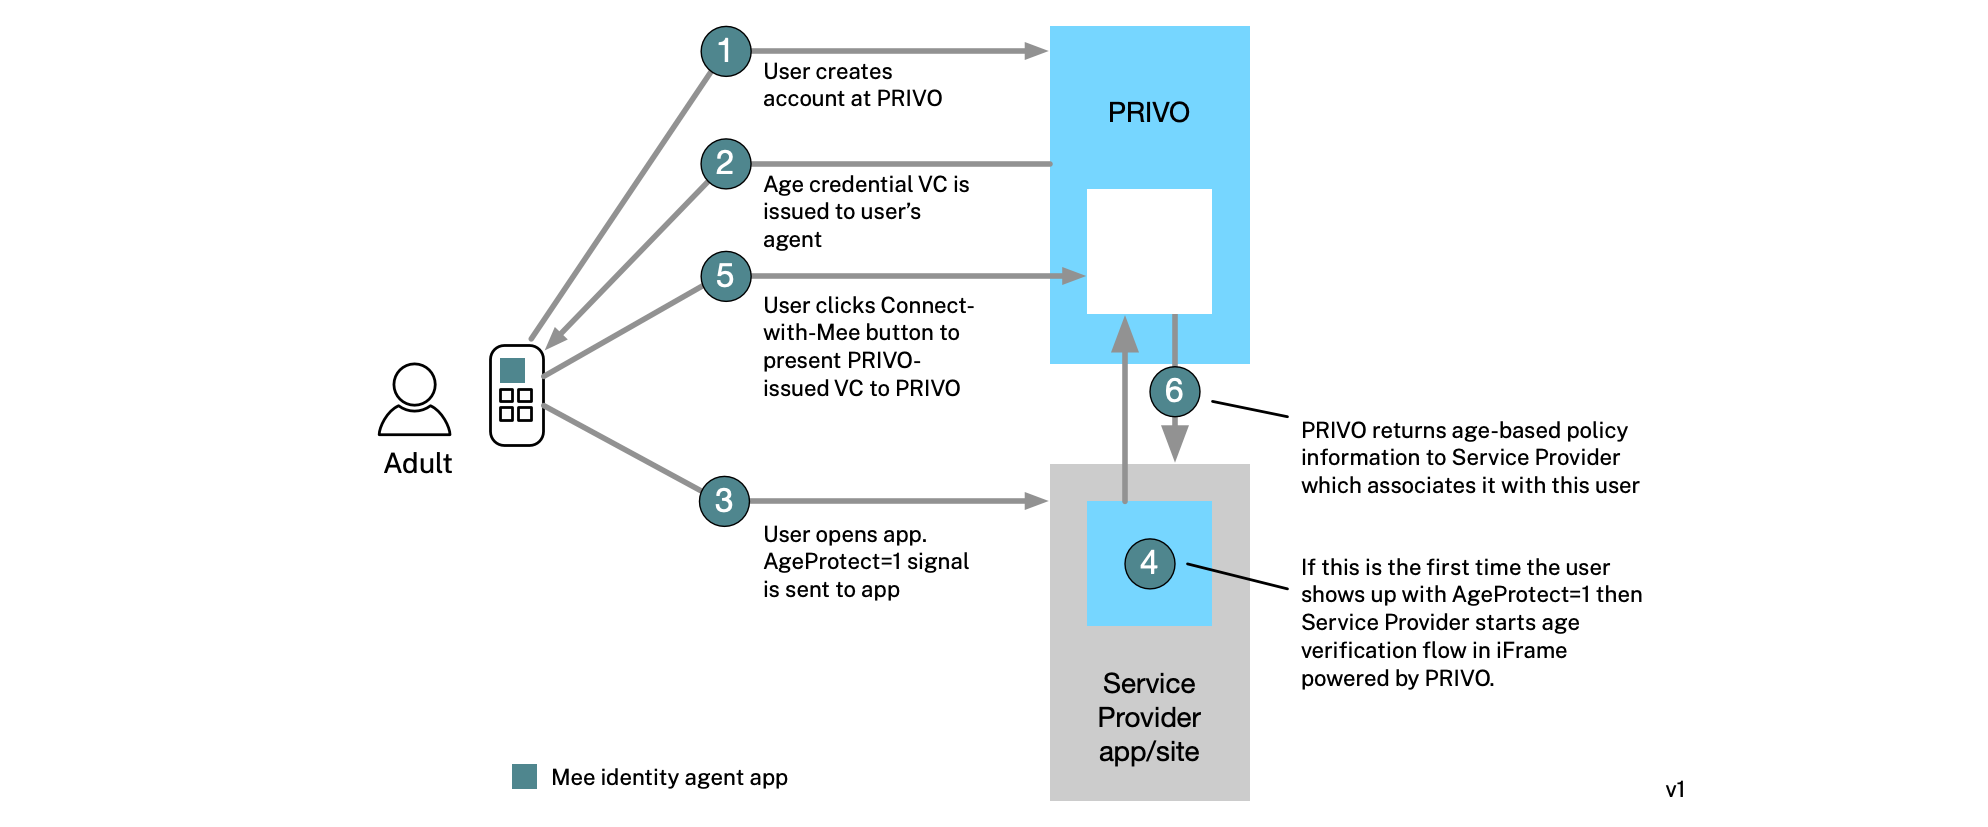
\includegraphics[width=\textwidth]{./images/adult.png}
	\caption{Adult gets AVR and visits an SP's website}
	\label{fig:adult}
\end{figure}

\begin{figure}
	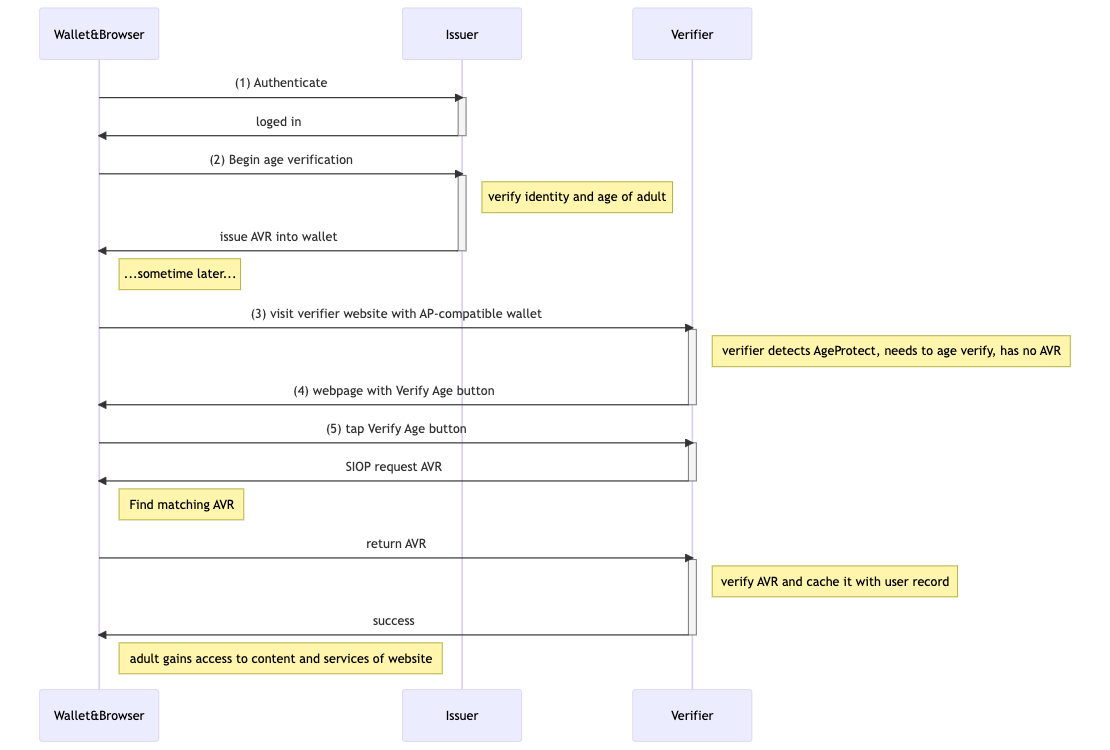
\includegraphics[width=\textwidth]{./images/adult-sequence.png}
	\caption{Adult gets AVR and visits an SP's website}
	\label{fig:adult-seq}
\end{figure}
\begin{comment}
MERMAID
sequenceDiagram
    participant Adult
    participant AVS
    participant ServiceProvider
    Adult->>+AVS: (1) visit AVS.com
    AVS->>-Adult: HTML page with AP-compatible button
    Adult->>+AVS: (2) tap AP-compatible button
    Note right of AVS: verify identity and age of adult
    AVS->>-Adult: issue AVR
    Note right of Adult: ...sometime later...
    Adult->>+ServiceProvider: (3) visit SP website for the first time (AP enabled)
    Note right of ServiceProvider: SP detects AgeProtect, needs to age verify, has no AVR
    ServiceProvider->>-Adult: (4) webpage with AP-compatible button
    Adult->>+ServiceProvider: (5) tap AP-compatible button
    ServiceProvider->>-Adult: SIOP request AVR
    Note right of Adult: Find matching AVR
    Adult->>ServiceProvider: return AVR
    Note right of ServiceProvider: verify AVR and cache it with user record
    Note right of ServiceProvider: adult gains access to content and services of website

\end{comment}

\subsection{Minor verifies age at a website}

In this scenario we show how a minor can verify their age at a website leveraging the fact that they were previously registered by a guardian at an AVS and issued with an AVR. In this scenario, the minor can take this AVR to any website without being tracked by the guardian or any other entity. 

The guardian registers a minor (e.g. child) at an AVS, shares a link (or QR code) with this minor, and the minor then visits a website that has implemented Age Protect. This flow, shown in Figure \ref{fig:guardian+minor}, has the following steps:
\begin{enumerate}
	\item The guardian goes to an AVS and taps an AP-compatible button. They then begin identity verification on themselves (using whatever methods are supported by the AVS) and then register the minor, a process that includes specifying the minor's birthdate.
	\item A link (and QR code) is generated for the minor and made available to the guardian.
	\item The guardian shares this link (or QR code) with the minor.
	\item The minor scans the QR code (or taps the URL) which brings them to the AVS. An AVR is issued and stored in their smartwallet.
	\item The minor goes to the SP's website. In the HTTP header the smartwallet includes field name of ``AgeProtect.''\footnote{The design of this field is under active development and thus may change} The SP detects this signal encoded in the header.
	\item If this is the first time that the minor has visited the site with AgeProtect enabled then the SP displays a page with an AP-compatible button prompting the minor to tap it and thereby request either an age-range or a birthdate.
	\item The minor taps an AP-compatible button and their smartwallet provides whatever age information the SP has requested: either an age-range derived from the AVR's birthdate or the actual birthdate itself.
\end{enumerate}

\begin{figure}
	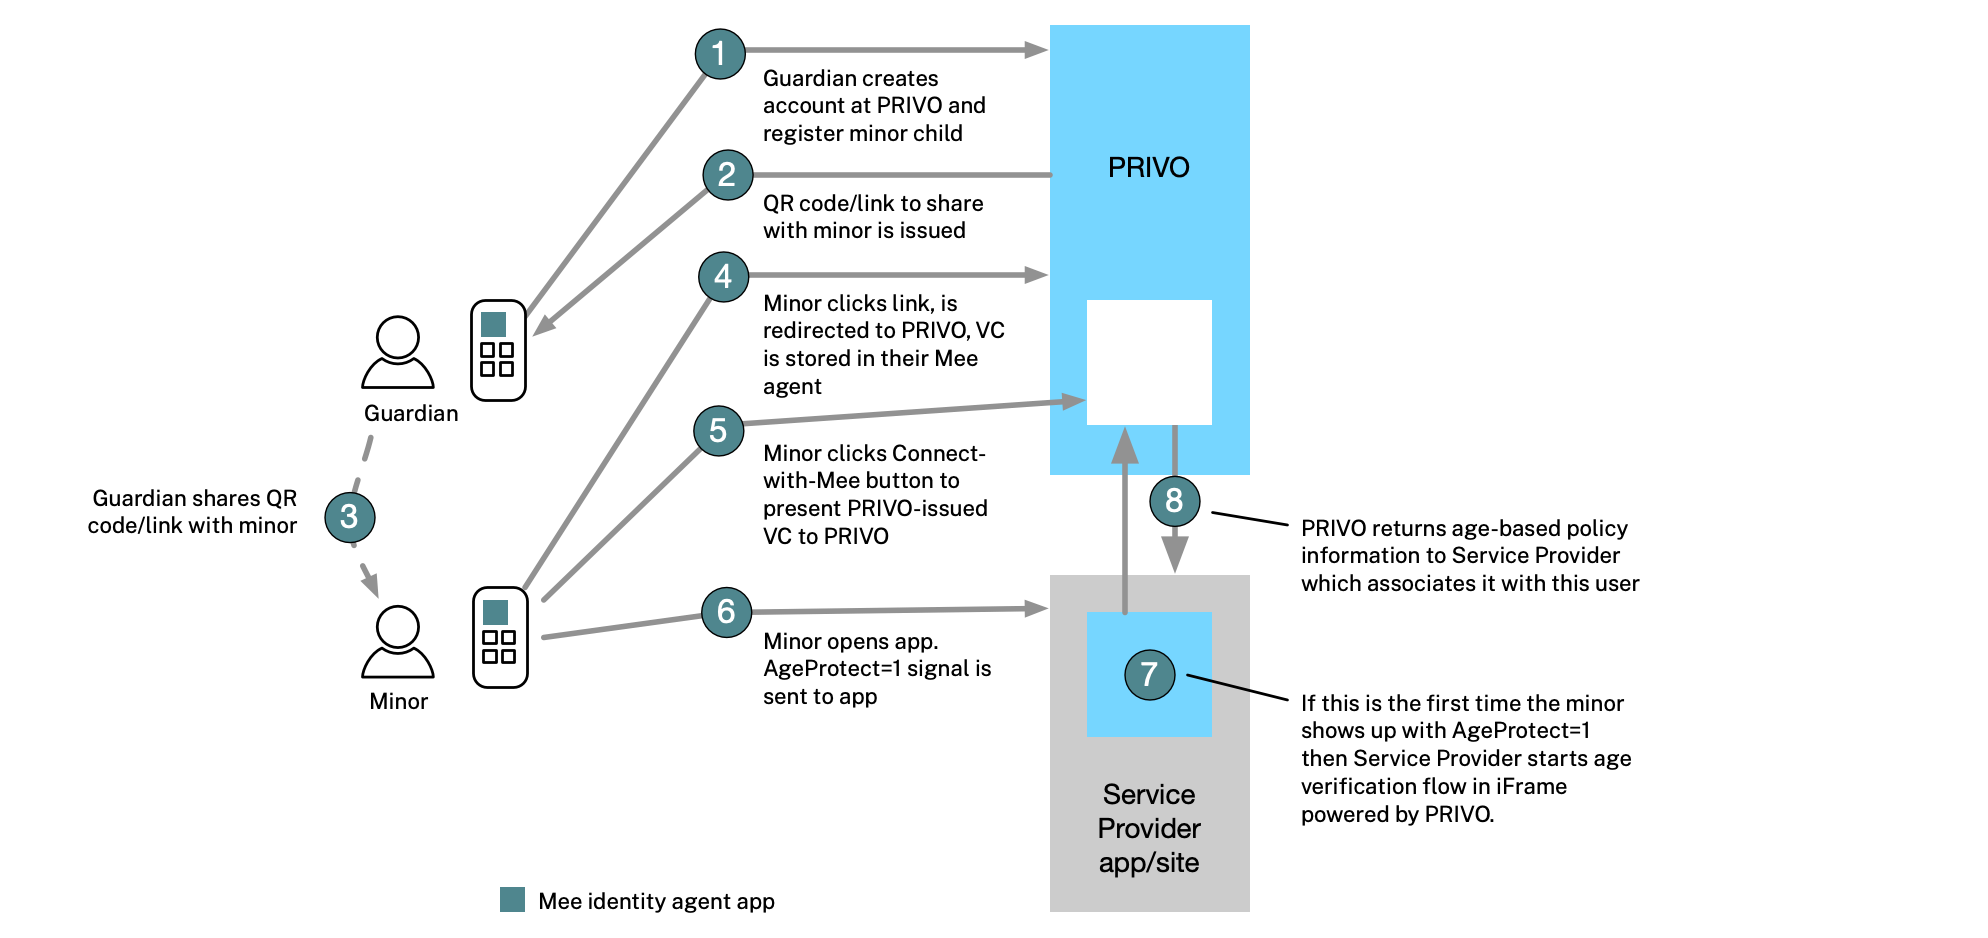
\includegraphics[width=\textwidth]{./images/guardian+minor.png}
	\caption{Minor with guardian flow}
	\label{fig:guardian+minor}
\end{figure}

\begin{comment}
\subsection{Consent: allowing/blocking access to a website by a minor}

In the previous scenario the minor was free to use any Age Protect website so long as the information in their AVR met the age criteria of the website. In this scenario we go further and show how the guardian can control the minor's access to specific websites and even specific kinds of services within a website (e.g. the ability to chat with others, upload images, etc.).

Here's a rough sketch of how this works. Every time the minor wishes to access a new website they must first possess (i.e. have stored in their smartwallet) an authorization token for it. For example if the minor wants to visit Facebook.com they must first have a token for Facebook.com. This token is issued by an interaction between the AVS and the guardian. 

Here's how the flow works the first time the minor attempts to go to Facebook.com: 
\begin{enumerate}
	\item Minor attempts to visit Facebook.com
	\item Their smartwallet's browser extension attepts to fetch from their smartwallet an authorization token (issued by an AVS) that specifies that the minor is permitted to visit Facebook.com. In this scenario no such token exists.
	\item The minor's smartwallet sends a request for authorization to the guardian's smartwallet (leveraging the digital connection between the guardian's smartwallet and the minor's smartwallet)
	\item The guardian's smartwallet invokes the AVS app/site. This app/site provides a UI that enables the guardian to manage an ``allowed list'' and a ``blocked list'' of SPs. Using this UI the guardian modifies these lists to allow or block access to Facebook.com. If access is allowed it generates a token encoding this capability. 
	\item The AVS issues the token to the guardian by adding it into a storage area within the guardian's smartwallet that is associated with the guardian's relationship with the AVS.
	\item The guardian's smartwallet sends this token to the minor's smartwallet (leveraging the digital connection between the guardian's smartwallet and the minor's smartwallet, [and specifically replication of the storage area in the guardian's smartwallet])
	\item The minor's smartwallet verifies this token and communicates with the browser extension to allow the browser to proceed to Facebook.com
\end{enumerate}
\end{comment}

\subsection{Minor uninstalls their smartwallet}

A minor can attempt to disable Age Protect by uninstalling the smartwallet from their devices. The smartwallet can, just before the uninstallation process completes, send a signal to the AVS. The AVS can in turn notify the minor's guardian that the minor is uninstalling Age Protect.


\section{Technical specifications}

This section is under development.

\subsection{Signaling protocol}
This subsection will describe the AppProtect=1 HTTP header field (which is identical in structure to the \hyperfootnote[Global Privacy Control][https://]{globalprivacycontrol.org}). We also need to develop a solution to send the Age Protect signal to mobile apps.

\subsection{AP-Compatible button}
This subsection will describe how an AP-Compatible button is to be implemented. It will extend the OpenID SIOPv2 spec. 

\subsection{Age Verification Record format}
This subsection will describe the schema of an AVR.\hyperfootnote[Verifiable Credential][https://]{w3.org/TR/vc-data-model/}

\subsection{Age Verification protocol}
This section will define the invocation flow, age verification claims (perhaps only user age range and jurisdiction), and mechanism for presenting/prove age with the AVR. 

\section{Initial implementation}

This section will describe an prototype implementation of Age Protect being developed by an AVS provider, \hyperfootnote[PRIVO][https://]{privo.com}, and smartwallet provider, \hyperfootnote[The Mee Foundation][https://]{mee.foundation}, and a software development firm, \hyperfootnote[Swift Invention.][https://]{swiftinvention.com}

\section{Conclusions and further work}
We have described the design of a new, opt-in, privacy-preserving age verification approach. This paper will be continuously updated as progress continues on the specifications and a prototype implementation.

\bibliography{../library}
\bibliographystyle{plainurl}
\end{document}  